\section{Numerical Integration} \label{S:5.6.NumInt}

\begin{goals}
\item How do we accurately evaluate a definite integral such as $\int_0^1 e^{-x^2} \, dx$ when we cannot use the First Fundamental Theorem of Calculus because the integrand lacks an elementary algebraic antiderivative?  Are there ways to generate accurate estimates without using extremely large values of $n$ in Riemann sums?
\item What is the Trapezoid Rule, and how is it related to left, right, and middle Riemann sums?
\item How are the errors in the Trapezoid Rule and Midpoint Rule related, and how can they be used to develop an even more accurate rule?
\item What role can a computer algebra system play in the process of finding antiderivatives?
\end{goals}

%--------------------------------------
% SUBSECTION INTRODUCTION
%--------------------------------------
\subsection*{Introduction}

When we were first exploring the problem of finding the net-signed area bounded by a curve, we developed the concept of a Riemann sum as a helpful estimation tool and a key step in the definition of the definite integral.  In particular, as we found in Section~\ref{S:4.2.Riemann}, recall that the left, right, and middle Riemann sums of a function $f$ on an interval $[a,b]$ are denoted $L_n$, $R_n$, and $M_n$, with formulas\small
\begin{equation} \label{E:Left}
L_n = f(x_0) \triangle x + f(x_1) \triangle x + \cdots + f(x_{n-1}) \triangle x = \sum_{i = 0}^{n-1} f(x_i) \triangle x,
\end{equation}
\begin{equation} \label{E:Left}R_n = f(x_1) \triangle x + f(x_2) \triangle x + \cdots + f(x_{n}) \triangle x = \sum_{i = 1}^{n} f(x_i) \triangle x,
\end{equation}
\begin{equation} \label{E:Left}M_n = f(\overline{x}_1) \triangle x + f(\overline{x}_2) \triangle x + \cdots + f(\overline{x}_{n}) \triangle x = \sum_{i = 1}^{n} f(\overline{x}_i) \triangle x,
\end{equation}\normalsize
where $x_0 = a$, $x_i = a + i\triangle x$, $x_n = b$, and $\triangle x = \frac{b-a}{n}$.  For the middle sum, note that $\overline{x}_{i} = (x_{i-1} + x_i)/2$.  

Further, recall that a Riemann sum is essentially a sum of (possibly signed) areas of rectangles, and that the value of $n$ determines the number of rectangles, while our choice of left endpoints, right endpoints, or midpoints determines how we use the given function to find the heights of the respective rectangles we choose to use.  Visually, we can see the similarities and differences among these three options in Figure~\ref{F:5.6.LRMsum}, where we consider the function $f(x) = -\frac{1}{20}(x-4)^3 + 7$ on the interval $[1,8]$, and use $5$ rectangles for each of the Riemann sums.

\begin{marginfigure} %MARGIN FIGURE
\margingraphics{figures/5_6_LRMsum.eps}
\caption{Left, right, and middle Riemann sums for $y = f(x)$ on $[1,8]$ with 5 subintervals.} \label{F:5.6.LRMsum}
\end{marginfigure}

While it is a good exercise to compute a few Riemann sums by hand, just to ensure that we understand how they work and how varying the function, the number of subintervals, and the choice of endpoints or midpoints affects the result, it is of course the case that using computing technology is the best way to determine $L_n$, $R_n$, and $M_n$ going forward.  Any computer algebra system will offer this capability; a straightforward option that happens to also be freely available online is the applet\footnote{Mike May, St.~Louis University, applet collection at \href{http://gvsu.edu/s/dQ}{\texttt{http://gvsu.edu/s/dQ}} building upon the work of David Eck \href{http://gvsu.edu/s/av}{\texttt{http://gvsu.edu/s/av}}.} at \href{http://gvsu.edu/s/dP}{\texttt{http://gvsu.edu/s/dP}}.  From this URL, we see the interface in Figure~\ref{F:5.6.MayApplet}.

\begin{marginfigure} %MARGIN FIGURE
\margingraphics{figures/5_6_MayApplet.pdf}
\caption{A snapshot of the applet for computing Riemann sums (and more) found at \href{http://gvsu.edu/s/dP}{\texttt{http://gvsu.edu/s/dP}}.} \label{F:5.6.MayApplet}
\end{marginfigure}

Note that we can adjust the formula for $f(x)$, the window of $x$- and $y$-values of interest, the number of subintervals, and the method.  The pictured result tells us that for $f(x) = x^2$ on the interval $[0,3]$ with 8 subintervals using the left endpoint rule, $\int_0^3 x^2 \, dx \approx L_8$, and $L_8 \approx 7.382815$.  

In what follows in this section we explore several different alternatives, including left, right, and middle Riemann sums, for estimating definite integrals.  One of our main goals is to develop formulas that enable us to estimate definite integrals accurately without having to use exceptionally large numbers of rectangles.

\begin{pa} \label{PA:5.6}
As we begin to investigate ways to approximate definite integrals, it will be insightful to compare results to integrals whose exact values we know.  To that end, the following sequence of questions centers on $\int_0^3 x^2 \, dx$. 
\ba
	\item Use the applet at \href{http://gvsu.edu/s/dP}{\texttt{http://gvsu.edu/s/dP}} with the function $f(x) = x^2$ on the window of $x$ values from $0$ to $3$ and $y$ values from $-1$ to $10$, to compute $L_3$, the left Riemann sum with three subintervals.
	\item Likewise, use the applet to compute $R_3$ and $M_3$, the right and middle Riemann sums with three subintervals, respectively.
	\item Use the Fundamental Theorem of Calculus to compute the exact value of $I = \int_0^3 x^2 \, dx$.
	\item We define the \emph{error} in an approximation of a definite integral to be the difference between the integral's exact value and the approximation's value.  What is the error that results from using $L_3$? From $R_3$?  From $M_3$?
	\item In what follows in this section, we will learn a new approach to estimating the value of a definite integral known as the Trapezoid Rule.  For now, use the ``Trapezoid'' option  in the applet in the pull-down menu for the ``Method'' of estimating the definite integral, and determine the approximation generated by 3 trapezoids.  What is the error in this approximation?  How does it compare to the errors you calculated in (d)?
	\item What is the formula for the area of a trapezoid with bases of length $b_1$ and $b_2$ and height $h$?
\ea
\end{pa} 
\afterpa %PREVIEW

\begin{example} \label{eg:5.6.1} % EXAMPLE
Approximate $\ds \int_0^1e^{-x^2}\ dx$ using the Left and Right Hand Rules with $5$ equally spaced subintervals.

\solution We begin by partitioning the interval $[0,1]$ into $5$ equally spaced intervals. We have $\dx = \frac{1-0}5 = 1/5=0.2$, so $$x_1 = 0,\ x_2 = 0.2,\ x_3 = 0.4,\ x_4 = 0.6,\ x_5 = 0.8,\ \text{and}\ x_6 = 1.$$

Using the Left Hand Rule, we have:

\begin{align*}
\sum_{i=1}^n f(x_i)\dx &= \big(f(x_1)+f(x_2) + f(x_3) + f(x_4) + f(x_5)\big)\dx \\
&= \big(f(0) + f(0.2) + f(0.4) + f(0.6) + f(0.8)\big)\dx \\
&\approx \big(1+0.961 + 0.852 + 0.698 + 0.527)(0.2)\\
&\approx 0.808.
\end{align*}

Using the Right Hand Rule, we have:

\begin{align*}
\sum_{i=1}^n f(x_{i+1})\dx &= \big(f(x_2) + f(x_3) + f(x_4) + f(x_5)+f(x_6)\big)\dx \\
&= \big(f(0.2) + f(0.4) + f(0.6) + f(0.8)+f(1)\big)\dx \\
&\approx \big(0.961 +0.852 + 0.698 + 0.527 + 0.368)(0.2)\\
&\approx 0.681.
\end{align*}

Figure~\ref{F:5-6-eg1} shows the rectangles used in each method to approximate the definite integral. These graphs show that in this particular case, the Left Hand Rule is an over approximation and the Right Hand Rule is an under approximation. To get a better approximation, we could use more rectangles. We could also average the Left and Right Hand Rule results together, giving $$ \frac{0.808 + 0.681}{2} = 0.7445.$$ The actual answer, accurate to $4$ places after the decimal, is $0.7468$, showing our average is a good approximation.
\end{example}

\begin{marginfigure}[-14cm] %MARGIN FIGURE
\subfloat[]{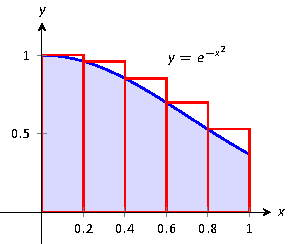
\includegraphics{figures/fignum1b}}

\subfloat[]{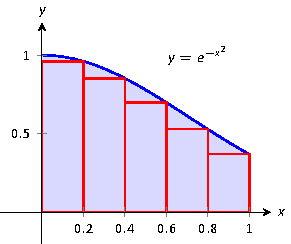
\includegraphics{figures/fignum1a}}
\caption{Approximating $\int_0^1e^{-x^2}\ dx$ in Example~\ref{eg:5.6.1}.}
\label{F:5-6-eg1}
\end{marginfigure} %EXAMPLE

%--------------------------------------
% SUBSECTION TRAPEZOID RULE
%--------------------------------------
\subsection*{The Trapezoid Rule} \index{trapezoid rule}

Throughout our work to date with developing and estimating definite integrals, we have used the simplest possible quadrilaterals (that is, rectangles) to subdivide regions with complicated shapes. It is natural, however, to wonder if other familiar shapes might serve us even better.  In particular, our goal is to be able to accurately estimate $\int_a^b f(x) \, dx$ without having to use extremely large values of $n$ in Riemann sums.

\begin{marginfigure}[2cm] %MARGIN FIGURE
\margingraphics{figures/5_6_TRAP.eps}
\caption{Estimating $\int_a^b f(x) \, dx$ using three subintervals and trapezoids, rather than rectangles, where $a = x_0$ and $b = x_3$.} 
\label{F:5.6.TRAP}
\end{marginfigure}

To this end, we consider an alternative to $L_n$, $R_n$, and $M_n$, know as the \emph{Trapezoid Rule}.  The fundamental idea is simple:  rather than using a rectangle to estimate the (signed) area \newline bounded by $y = f(x)$ on a small interval, we use a trapezoid.  For example, in Figure~\ref{F:5.6.TRAP}, we estimate the area under the pictured curve using three subintervals and the trapezoids that result from connecting the corresponding points on the curve with straight lines.

The biggest difference between the Trapezoid Rule and a left, right, or middle Riemann sum is that on each subinterval, the Trapezoid Rule uses two function values, rather than one, to estimate the (signed) area bounded by the curve.  For instance, to compute $D_1$, the area of the trapezoid generated by the curve $y = f(x)$ in Figure~\ref{F:5.6.TRAP} on $[x_0, x_1]$, we observe that the left base of this trapezoid has length $f(x_0)$, while the right base has length $f(x_1)$.  In addition, the height of this trapezoid is $x_1 - x_0 = \triangle x = \frac{b-a}{3}$.  Since the area of a trapezoid is the average of the bases times the height, we have
$$D_1 = \frac{1}{2}(f(x_0) + f(x_1)) \cdot \triangle x.$$
Using similar computations for $D_2$ and $D_3$, we find that $T_3$, the trapezoidal approximation to $\int_a^b f(x) \, dx$ is given by \small
%\begin{align*}
\[T_3  =  D_1 + D_2 + D_3 \]
\[=   \frac{1}{2}(f(x_0) + f(x_1)) \cdot \triangle x +  \frac{1}{2}(f(x_1) + f(x_2)) \cdot \triangle x  +  \frac{1}{2}(f(x_2) + f(x_3)) \cdot \triangle x.\] \normalsize
%	& =   \frac{1}{2}(f(x_0) + f(x_1)) \cdot \triangle x \\
%	& +  \frac{1}{2}(f(x_1) + f(x_2)) \cdot \triangle x \\
%	& +  \frac{1}{2}(f(x_2) + f(x_3)) \cdot \triangle x.
%\end{align*}
Because both left and right endpoints are being used, we can recognize within the trapezoidal approximation the use of both left and right Riemann sums.  In particular, rearranging the expression for $T_3$ by removing a factor of $\frac{1}{2}$, then grouping all of the left endpoint evaluations of $f$, and then grouping all of the right endpoint evaluations of $f$, we have equivalently that \small
\begin{equation} \label{E:Trap3}
T_3 =  \frac{1}{2} \left[ (f(x_0) \triangle x + f(x_1) \triangle x + f(x_2) \triangle x)  + (f(x_1) \triangle x + f(x_2) \triangle x + f(x_3) \triangle x) \right].
\end{equation}\normalsize
At this point, we observe that two familiar sums have arisen.  Since the left Riemann sum is $L_3 = f(x_0) \triangle x + f(x_1) \triangle x + f(x_2)$, and the right Riemann sum is $R_3 = f(x_1) \triangle x + f(x_2) \triangle x + f(x_3) \triangle x$, substituting $L_3$ and $R_3$ for the corresponding expressions in Equation~\ref{E:Trap3}, it follows that
$$T_3 = \frac{1}{2} \left[ L_3 + R_3 \right].$$
We have thus seen the main ideas behind a very important result:  using trapezoids to estimate the (signed) area bounded by a curve is the same as averaging the estimates generated by using left and right endpoints.

\concept{The Trapezoid Rule}{  %CONCEPT
The trapezoidal approximation, $T_n$, of the definite integral $\int_a^b f(x) \, dx$ using $n$ subintervals is given by the rule
\begin{eqnarray*}
T_n & = & \frac{1}{2}(f(x_0) + f(x_1)) \triangle x + \frac{1}{2}(f(x_1) + f(x_2)) \triangle x \\
& & + \cdots + \frac{1}{2}(f(x_{n-1}) + f(x_n)) \triangle x. \\
	& =  & \sum_{i=0}^{n-1} \frac{1}{2}(f(x_i) + f(x_{i+1})) \triangle x.
\end{eqnarray*}
Moreover, with $L_n$ and $R_n$ representing the familiar left and right Riemann sums for estimating the same definite integral, it follows that
$$T_n = \frac{1}{2} \left[ L_n + R_n \right].$$
} %end CONCEPT

\begin{marginfigure}[8cm] %MARGIN FIGURE
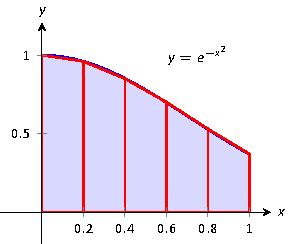
\includegraphics{figures/fignum3a} %Example 134 APEX
\caption{Approximating $\int_0^1 e^{-x^2}\ dx$ using 5 trapezoids of equal widths.}
\label{F:5-6-EG2}
\end{marginfigure}

\begin{margintable} %MARGIN TABLE
\begin{center}
\caption{A table of values of $e^{-x^2}$.} 
\label{T:5-6-EG2} 
\begin{tabular}{cc}
$x_i$ & $e^{-x_i^2}$ \\ \hline
$0$ & 1\\
$0.2$ & $0.961$ \\
$0.4$ & $0.852$ \\
$0.6$ & $0.698$ \\
$0.8$ & $0.527$ \\
$1$ & $0.368$
\end{tabular}
\end{center}
\end{margintable}


\begin{example} \label{eg:5.6.2} % EXAMPLE
Use $5$ trapezoids of equal width to approximate $\ds \int_0^1e^{-x^2}\ dx$.

\solution To compute the areas of the $5$ trapezoids in Figure \ref{F:5-6-EG2}, it will again be useful to create a table of values as shown in Table \ref{T:5-6-EG2}. The leftmost trapezoid has legs of length $1$ and $0.961$ and a height of $0.2$. Thus, by our formula, the area of the leftmost trapezoid is: 
$$ \frac{1+0.961}{2}(0.2) = 0.1961.$$
Moving right, the next trapezoid has legs of length $0.961$ and $0.852$ and a height of $0.2$. Thus its area is: $$\frac{0.961+0.852}2(0.2) = 0.1813.$$

The sum of the areas of all $5$ trapezoids is:
\begin{align*}
\frac{1+0.961}{2}(0.2) + \frac{0.961+0.852}2(0.2)+\frac{0.852+0.698}2(0.2)&+ \\
\frac{0.698+0.527}2(0.2)+\frac{0.527+0.368}2(0.2)&= 0.7445.
\end{align*}

Alternatively, if we use the Trapezoid Rule with $n=5$ along with the results from Example~\ref{eg:5.6.1}, we have
\[ T_5  =  \frac{1}{2}\Big[L_5 + R_5 \Big] \approx \frac{1}{2}\Big[ 0.808 + 0.681 \Big] \approx 0.7445 \]
We approximate $\ds \int_0^1 e^{-x^2}\ dx \approx 0.7445.$
\end{example}

 %EXAMPLE

\begin{activity} \label{A:5.6.1}  In this activity, we explore the relationships among the errors generated by left, right, midpoint, and trapezoid approximations to the definite integral $\int_1^2 \frac{1}{x^2} \, dx$. 
\ba
	\item Use the First FTC to evaluate $\int_1^2 \frac{1}{x^2} \, dx$ exactly.
	\item Use appropriate computing technology to compute the following approximations for $\int_1^2 \frac{1}{x^2} \, dx$:  $T_4$, $M_4$, $T_8$, and $M_8$.  
	\item Let the \emph{error} \index{error} \index{trapezoid rule!error} \index{midpoint rule!error} of an approximation be the difference between the exact value of the definite integral and the resulting approximation.  For instance, if we let $E_{T,4}$ represent the error that results from using the trapezoid rule with $4$ subintervals to estimate the integral, we have 
	$$E_{T,4} = \int_1^2 \frac{1}{x^2} \, dx -  T_4.$$
	Similarly, we compute the error of the midpoint rule approximation with 8 subintervals by the formula
	$$E_{M,8} = \int_1^2 \frac{1}{x^2} \, dx -  M_8.$$
	Based on your work in (a) and (b) above, compute $E_{T,4}$, $E_{T,8}$, $E_{M,4}$, $E_{M,8}$.
	\item Which rule consistently over-estimates the exact value of the definite integral?  Which rule consistently under-estimates the definite integral?
	\item What behavior(s) of the function $f(x) = \frac{1}{x^2}$ lead to your observations in (d)?
\ea
\end{activity}
\begin{smallhint}
\ba
	\item Small hints for each of the prompts above.
\ea
\end{smallhint}
\begin{bighint}
\ba
	\item Big hints for each of the prompts above.
\ea
\end{bighint}
\begin{activitySolution}
\ba
	\item Solutions for each of the prompts above.
\ea
\end{activitySolution}
\aftera % ACTIVITY

%---------------------------------------------------
% SUBSECTION COMPARING MIDPOINT AND TRAPEZOID RULE
%---------------------------------------------------
\subsection*{Comparing the Midpoint and Trapezoid Rules}

We know from the definition of the definite integral of a continuous function $f$, that if we let $n$ be large enough, we can make the value of any of the approximations $L_n$, $R_n$, and $M_n$ as close as we'd like (in theory) to the exact value of $\int_a^b f(x) \, dx$.  Thus, it may be natural to wonder why we ever use any rule other than $L_n$ or $R_n$ (with a sufficiently large $n$ value) to estimate a definite integral.  One of the primary reasons is that as $n \to \infty$, $\triangle x = \frac{b-a}{n} \to 0$, and thus in a Riemann sum calculation with a large $n$ value, we end up multiplying by a number that is very close to zero.  Doing so often generates roundoff error, as representing numbers close to zero accurately is a persistent challenge for computers.

Hence, we are exploring ways by which we can estimate definite integrals to high levels of precision, but without having to use extremely large values of $n$.  Paying close attention to patterns in errors, such as those observed in Activity~\ref{A:5.6.1}, is one way to begin to see some alternate approaches.

To begin, we make a comparison of the errors in the Midpoint and Trapezoid rules from two different perspectives.  First, consider a function of consistent concavity on a given interval, and picture approximating the area bounded on that interval by both the Midpoint and Trapezoid rules using a single subinterval.

\begin{marginfigure} %MARGIN FIGURE
\margingraphics{figures/5_6_MidVTrap.eps}
\caption{Estimating $\int_a^b f(x) \, dx$ using a single subinterval: at left, the trapezoid rule; in the middle, the midpoint rule; at right, a modified way to think about the midpoint rule.} 
\label{F:5.6.MidVTrap}
\end{marginfigure}

As seen in Figure~\ref{F:5.6.MidVTrap}, it is evident that whenever the function is concave up on an interval, the Trapezoid Rule with one subinterval, $T_1$, will overestimate the exact value of the definite integral on that interval.  Moreover, from a careful analysis of the line that bounds the top of the rectangle for the Midpoint Rule (shown in magenta), we see that if we rotate this line segment until it is tangent to the curve at the point on the curve used in the Midpoint Rule (as shown at right in Figure~\ref{F:5.6.MidVTrap}), the resulting trapezoid has the same area as $M_1$, and this value is less than the exact value of the definite integral.  Hence, when the function is concave up on the interval, $M_1$ underestimates the integral's true value.

These observations extend easily to the situation where the function's concavity remains consistent but we use higher values of $n$ in the Midpoint and Trapezoid Rules.  Hence, whenever $f$ is concave up on $[a,b]$, $T_n$ will overestimate the value of $\int_a^b f(x) \, dx$, while $M_n$ will underestimate $\int_a^b f(x) \, dx$.   The reverse observations are true in the situation where $f$ is concave down.

Next, we compare the size of the errors between $M_n$ and $T_n$.  Again, we focus on $M_1$ and $T_1$ on an interval where the concavity of $f$ is consistent.  In Figure~\ref{F:5.6.MidTrapError}, the error of the Trapezoid Rule is shaded in red, while the error of the Midpoint Rule is shaded lighter red.  

\begin{marginfigure} %MARGIN FIGURE
\margingraphics{figures/5_6_MidTrapError.eps}
\caption{Comparing the error in estimating $\int_a^b f(x) \, dx$ using a single subinterval: in red, the error from the Trapezoid rule; in light red, the error from the Midpoint rule.} 
\label{F:5.6.MidTrapError}
\end{marginfigure}

It is visually apparent that the error in the Trapezoid Rule is more significant.  To see how much more significant, let's consider two examples and some particular computations.  If we let $f(x) = 1-x^2$ and consider $\int_0^1 f(x) \,dx$, we know by the First FTC that the exact value of the integral is
$$\int_0^1 (1-x^2) \, dx = x - \frac{x^3}{3} \bigg\vert_0^1 = \frac{2}{3}.$$
Using appropriate technology to compute $M_4$, $M_8$, $T_4$, and $T_8$, as well as the corresponding errors $E_{M,4}$, $E_{M,8}$, $E_{T,4}$, and $E_{T,8}$, as we did in Activity~\ref{A:5.6.1}, we find the results summarized in Table~\ref{T:5.6.Ex2}.  Note that in the table, we also include the approximations and their errors for the example $\int_1^2 \frac{1}{x^2} \, dx$ from Activity~\ref{A:5.6.1}.

Recall that for a given function $f$ and interval $[a,b]$, $E_{T,4} = \int_a^b f(x) \,dx - T_4$ calculates the difference between the exact value of the definite integral and the approximation generated by the Trapezoid Rule with $n = 4$.  If we look at not only $E_{T,4}$, but also the other errors generated by using $T_n$ and $M_n$ with $n = 4$ and $n = 8$ in the two examples noted in Table~\ref{T:5.6.Ex2}, we see an evident pattern.  Not only is the sign of the error (which measures whether the rule generates an over- or under-estimate) tied to the rule used and the function's concavity, but the magnitude of the errors generated by $T_n$ and $M_n$ seems closely connected.  In particular, the errors generated by the Midpoint Rule seem to be about half the size of those generated by the Trapezoid Rule. 

\begin{table}[h]\small
\begin{center}
\begin{tabularx}{\textwidth}{|X|l|r||l|r|}
\hline
\T \ & $\int_0^1 (1-x^2) \ dx = 0.\overline{6} $ & \multicolumn{1}{c||}{error} & $\int_1^2 \frac{1}{x^2} \ dx = 0.5$ & \multicolumn{1}{c|}{error} \B \\
\hline \hline
\T $T_4$ & $0.65625$ & $-0.01041667$ & $0.50899376$ & $0.00899376$ \B \\
\hline
\T $M_4$ & $0.671875$ & $0.00520833$ & $0.49554794$ & $-0.00445206$ \B \\
\hline
\T $T_8$ & $0.6640625$ & $-0.00260417$ & $0.50227085$ & $0.00227085$ \B \\
\hline
\T $M_8$ & $0.66796875$ & $0.00130208$ & $0.49886749$ & $-0.00113251$ \B \\
\hline
\end{tabularx}
\end{center}
\caption{Calculations of $T_4$, $M_4$, $T_8$, and $M_8$, along with corresponding errors, for the definite integrals $\int_0^1 (1-x^2) \ dx$ and $\int_1^2 \frac{1}{x^2} \ dx$.}
\label{T:5.6.Ex2}
\end{table}\normalsize

That is, we can observe in both examples that $E_{M,4} \approx -\frac{1}{2} E_{T,4}$ and $E_{M,8} \approx -\frac{1}{2}E_{T,8}$, which demonstrates a property of the Midpoint and Trapezoid Rules that turns out to hold in general: for a function of consistent concavity, the error in the Midpoint Rule has the opposite sign and approximately half the magnitude of the error of the Trapezoid Rule.  Said symbolically,
$$E_{M,n} \approx -\frac{1}{2} E_{T,n}.$$
This important relationship suggests a way to combine the Midpoint and Trapezoid Rules to create an even more accurate approximation to a definite integral.

%--------------------------------------
% SUBSECTION SIMPSON'S RULE
%--------------------------------------
\subsection*{Simpson's Rule} \index{Simpson's rule}  %FIX TO USE PARABOLAS

When we first developed the Trapezoid Rule, we observed that it can equivalently be viewed as resulting from the average of the Left and Right Riemann sums:
$$T_n = \frac{1}{2}(L_n + R_n).$$
Whenever a function is always increasing or always decreasing on the interval $[a,b]$, one of $L_n$ and $R_n$ will over-estimate the true value of $\int_a^b f(x) \, dx$, while the other will under-estimate the integral.  Said differently, the errors found in $L_n$ and $R_n$ will have opposite signs; thus, averaging $L_n$ and $R_n$ eliminates a considerable amount of the error present in the respective approximations.  In a similar way, it makes sense to think about averaging $M_n$ and $T_n$ in order to generate a still more accurate approximation.

At the same time, we've just observed that $M_n$ is typically about twice as accurate as $T_n$.  Thus, we instead choose to use the weighted average \index{weighted average}
\begin{equation} \label{E:Simpson}
S_n = \frac{2M_n + T_n}{3}.
\end{equation}
The rule for $S_n$ giving by Equation~\ref{E:Simpson} is usually known as \emph{Simpson's Rule}. Thomas Simpson was an 18th century mathematician; his idea was to extend the Trapezoid rule, but rather than using straight lines to build trapezoids, to use quadratic functions to build regions whose area was bounded by parabolas (whose areas he could find exactly). Figure \ref{F:5.6.simpson} is an example of approximating a function with parabolas. 

\begin{figure} % FIGURE
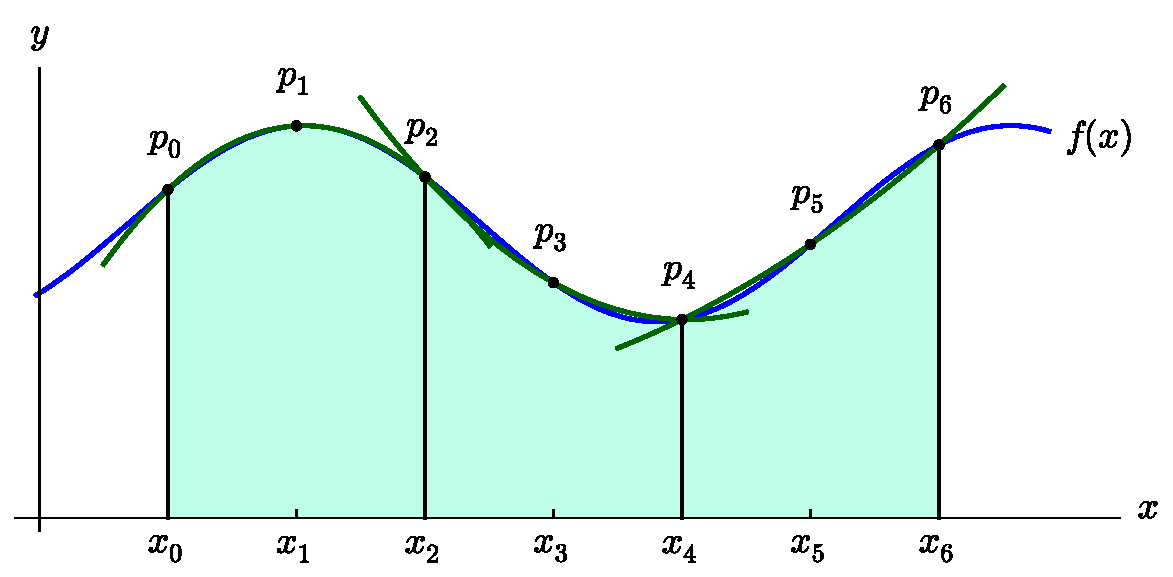
\includegraphics[width=\textwidth]{figs/5/simpson.pdf}
\caption{Approximating the area underneath a function using parabolas.}
\label{F:5.6.simpson}
\end{figure}

In general, the equation of a parabola is given by $y=Ax^2+Bx+C$. If we have three points $P_0$, $P_1$, and $P_2$, we can find $A$, $B$, and $C$ so that the points $P_0$, $P_1$, and $P_2$ lie on the graph of the parabola. To simplify the calculations, we consider the interval $[-\Delta x, \Delta x]$ and the corresponding points on the curve $P_0(-\Delta x, y_0)$, $P_1(0,y_1)$, and $P_2(\Delta x, y_2)$. This choice of points splits the interval into two eqaul subintervals. The area under the parabola and above $[-\Delta x, \Delta x]$ is obtained by evaluating

\begin{marginfigure} % MARGIN FIGURE
\margingraphics{figs/5/simpsonb.pdf} 
\caption{Consider the interval $[-\Delta x, \Delta x]$ and the corresponding points on the curve $P_0(-\Delta x, y_0)$, $P_1(0,y_1)$, and $P_2(\Delta x, y_2)$.}
\label{F:5.6.simpsonb}
\end{marginfigure}

\begin{align*}
 \text{Area} = & \int_{-\Delta x}^{\Delta x} Ax^2+Bx+C \, dx = \frac{Ax^3}{3}+\frac{Bx^2}{2}+Cx \Big\vert_{-\Delta x}^{\Delta x} \\
 =& \ 2 \Big( \frac{A(\Delta x)^3}{3} + C\Delta x\Big) = \frac{\Delta x}{3}( 2A(\Delta x)^2 + 6C)
\end{align*}
Since the parabola passes through the points $P_0$, $P_1$, and $P_2$, we know the coordinates of the points must satisfy $y=Ax^2+Bx+C$. Thus, we obtain 
\begin{align*}
y_0 =& \  A(\Delta x)^2 - B \Delta x + C \\
y_1 =& \ C \\
y_2 =& \ A(\Delta x)^2 + B \Delta x + C
\end{align*}     
Adding the first and third equations to $4$ times the second equation, we have 
$$ y_0 + 4y_1 + y_2 = 2A(\Delta x)^2 + 6C $$
Therefore, the area under the parabola is $\frac{\Delta x}{3}(y_0 + 4y_1 + y_2)$.

The area only depends on the $y$-coordinates of the three points. We get a similar expression for approximating the area under $f(x)$ above any interval $[a,b]$.\small
$$ \frac{\Delta x}{3}(y_0 + 4y_1 + y_2) + \frac{\Delta x}{3}(y_2 + 4y_3 + y_4) + \cdots + \frac{\Delta x}{3}(y_{N-2} + 4y_{N-1} + y_N)$$\normalsize
Simplifying we get Simpson's Rule, which we state here as a concept.

\concept{Simpson's Rule} % CONCEPT   
{Let $N$ be an even integer. Suppose $f$ is defined and integrable on $[a,b]$. The Simpson's Rule approximation to $\int_a^b f(x) \, dx$ using $N$ equally spaced subintervals on $[a,b]$ is \small
$$ S_N = \frac{\Delta x}{3} \Big( f(x_0) + 4f(x_1) + 2f(x_2) + 4f(x_3) + \cdots + 4f(x_{N-1}) + f(x_N) \Big) $$ \normalsize
Alternatively, if Midpoint and Trapezoid approximations are known, 
$$S_N = \frac{2M_N + T_N}{3}. $$
} % end CONCEPT

We build upon the results in Table~\ref{T:5.6.Ex2} to see the approximations generated by Simpson's Rule.  In particular, in Table~\ref{T:5.6.Ex3}, we include all of the results in Table~\ref{T:5.6.Ex2}, but include additional results for $\ds S_4 = \frac{2M_4 + T_4}{3}$ and $\ds S_8 = \frac{2M_8 + T_8}{3}$.

The results seen in Table~\ref{T:5.6.Ex3} are striking.  If we consider the $S_8$ approximation of $\ds\int_1^2 \frac{1}{x^2} \, dx$, the error is only $E_{S,8} = 0.0000019434$.  By contrast, $L_8 = 0.5491458502$, so the error of that estimate is $E_{L,8} = -0.0491458502$.  Moreover, we observe that generating the approximations for Simpson's Rule is almost no additional work:  once we have $L_n$, $R_n$, and $M_n$ for a given value of $n$, it is a simple exercise to generate $T_n$, and from there to calculate $S_n$.  The error in the Simpson's Rule approximations of $\int_0^1 x^2 \, dx$ is even smaller.

\begin{table}[h]\small
\begin{center}
\begin{tabularx}{\textwidth}{|X|l|r||l|r|}
\hline
\T \ & $\int_0^1 (1-x^2) \ dx = 0.\overline{6} $ & \multicolumn{1}{c||}{error} & $\int_1^2 \frac{1}{x^2} \ dx = 0.5$ & \multicolumn{1}{c|}{error} \B \\
\hline \hline
\T $T_4$ & $0.65625$ & $-0.01041667$ & $0.50899376$ & $0.00899376$ \B \\
\hline
\T $M_4$ & $0.671875$ & $0.00520833$ & $0.49554794$ & $-0.00445206$ \B \\
\hline
\T $S_4$ & $0.6666666668$ & $10^{-10}$ & $0.50002988$ & $0.00002988$ \B \\
\hline
\T $T_8$ & $0.6640625$ & $-0.00260417$ & $0.50227085$ & $0.00227085$ \B \\
\hline
\T $M_8$ & $0.66796875$ & $0.00130208$ & $0.49886749$ & $-0.00113251$ \B \\
\hline
\T $S_8$ & $0.6666666667$ &  $0$ & $40.50000194$ & $0.00000194$ \B \\
\hline
\end{tabularx} 
\end{center}
\caption{Table~\ref{T:5.6.Ex2} updated to include $S_4$, $S_8$, and the corresponding errors.} \label{T:5.6.Ex3}
\end{table}\normalsize

\begin{margintable}[6cm] %MARGIN TABLE
\begin{center}
\caption{A table of values of $e^{-x^2}$.} 
\label{T:5-6-EG3} 
\begin{tabular}{cc}
$x_i$ & $e^{-x_i^2}$ \\ \hline
$0$ & $1$\\
$0.25$ & $0.939$ \\
$0.5$ & $0.779$ \\
$0.75$ & $0.570$ \\
$1$ & $0.368$\\
\end{tabular}
\end{center}
\end{margintable}


\begin{example} \label{eg:5.6.3} % EXAMPLE
Approximate $\ds\int_0^1 e^{-x^2}\ dx$ using Simpson's Rule and $4$ equally spaced subintervals.

\solution We begin by making a table of values as we have in the past, as shown in Table~\ref{T:5-6-EG3}.

Simpson's Rule states that $$\int_0^1e^{-x^2}\ dx \approx \frac{0.25}{3}\Big[1+4(0.939)+2(0.779)+4(0.570) + 0.368\Big] = 0.7468\overline{3}.$$

Recall in Example \ref{eg:5.6.2} we stated that the correct answer, accurate to $4$ places after the decimal, was $0.7468$. Our approximation with Simpson's Rule, with $4$ subintervals, is better than our approximation with the Trapezoidal Rule using $5$.

Figure~\ref{F:5-6-EG3} shows $f(x) = e^{-x^2}$ along with its approximating parabolas, demonstrating how good our approximation is. The approximating curves are nearly indistinguishable from the actual function.
\end{example}

\begin{marginfigure}[-1cm] %MARGIN FIGURE
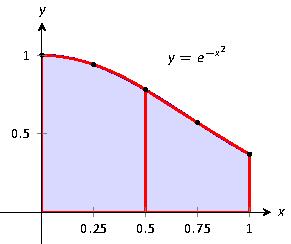
\includegraphics{figures/fignum5b} %Example 136 APEX
\caption{Approximating $\int_0^1 e^{-x^2}\ dx$ using Simpson's Rule.}
\label{F:5-6-EG3}
\end{marginfigure} %EXAMPLE

These rules are not only useful for approximating definite integrals such as $\int_0^1 e^{-x^2} \, dx$, for which we cannot find an elementary antiderivative of $e^{-x^2}$, but also for approximating definite integrals in the setting where we are given a function through a table of data.

Similar to how the Midpoint and Trapezoid approximations are exact for linear functions, Simpson's Rule approximations are exact for quadratic and cubic functions.  See additional discussion on this issue later in the section and in the exercises.



\begin{activity} \label{A:5.6.2}  A car traveling along a straight road is braking and its velocity is measured at several different points in time, as given in the following table.  Assume that $v$ is continuous, always decreasing, and always decreasing at a decreasing rate, as is suggested by the data.
\begin{center}
\begin{tabular}{|l|c|c|c|c|c|c|c|}
\hline
seconds, $t$ & $0$ & $0.3$ & $0.6$ & $0.9$ & $1.2$ & $1.5$ & $1.$8 \\
\hline
Velocity in ft/sec, $v(t)$ & $100$ & $99$ & $96$ & $90$ & $80$ & $50$ & $0$ \\
\hline
\end{tabular}
\end{center}
\ba
	\item Plot the given data on the set of axes provided in Figure~\ref{F:5.6.Act2} with time on the horizontal axis and the velocity on the vertical axis.
	\item What definite integral will give you the exact distance the car traveled on $[0,1.8]$?
	\item Estimate the total distance traveled on $[0,1.8]$ by computing $L_3$, $R_3$, and $T_3$.  Which of these under-estimates the true distance traveled?
	\item Estimate the total distance traveled on $[0,1.8]$ by computing $M_3$.  Is this an over- or under-estimate?  Why?
	\item Use your results from (c) and (d) improve your estimate further by using Simpson's Rule.
	\item What is your best estimate of the average velocity of the car on $[0,1.8]$?  Why?  What are the units on this quantity?
\ea

\end{activity}

\begin{marginfigure}[-6cm]
\margingraphics{figures/5_6_Act2.eps}
\caption{Axes for plotting the data in Activity~\ref{A:5.6.2}.} 
\label{F:5.6.Act2}
\end{marginfigure}
\begin{smallhint}
\ba
	\item Small hints for each of the prompts above.
\ea
\end{smallhint}
\begin{bighint}
\ba
	\item Big hints for each of the prompts above.
\ea
\end{bighint}
\begin{activitySolution}
\ba
	\item Solutions for each of the prompts above.
\ea
\end{activitySolution}
\aftera % ACTIVITY

%--------------------------------------------------------------------------------------------------------
% SUBSECTION OVERALL OBSERVATIONS REGARDING L_N, R_N, T_N, M_N, AND S_N
%--------------------------------------------------------------------------------------------------------
\subsection*{Overall observations regarding $L_n$, $R_n$, $T_n$, $M_n$, and $S_n$.}

As we conclude our discussion of numerical approximation of definite integrals, it is important to summarize general trends in how the various rules over- or under-estimate the true value of a definite integral, and by how much.  To revisit some past observations and see some new ones, we consider the following activity.

\begin{marginfigure}[6cm]
\margingraphics{figures/5_6_Act3.eps}
\caption{Axes for plotting the functions in Activity~\ref{A:5.6.3}.} 
\label{F:5.6.Act3}
\end{marginfigure}

\begin{activity} \label{A:5.6.3}  Consider the functions $f(x) = 2-x^2$, $g(x) = 2-x^3$, and $h(x) = 2-x^4$, all on the interval $[0,1]$.  For each of the questions that require a numerical answer in what follows, write your answer exactly in fraction form.
\ba
	\item On the three sets of axes provided in Figure~\ref{F:5.6.Act3}, sketch a graph of each function on the interval $[0,1]$, and compute $L_1$ and $R_1$ for each.  What do you observe?
	\item Compute $M_1$ for each function to approximate $\int_0^1 f(x) \,dx$, $\int_0^1 g(x) \,dx$, and $\int_0^1 h(x) \,dx$, respectively.
	\item Compute $T_1$ for each of the three functions, and hence compute $S_1$ for each of the three functions.
	\item Evaluate each of the integrals $\int_0^1 f(x) \,dx$, $\int_0^1 g(x) \,dx$, and $\int_0^1 h(x) \,dx$ exactly using the First FTC.
	\item For each of the three functions $f$, $g$, and $h$, compare the results of $L_1$, $R_1$, $M_1$, $T_1$, and $S_1$ to the true value of the corresponding definite integral.  What patterns do you observe?
\ea

\end{activity}
\begin{smallhint}
\ba
	\item Small hints for each of the prompts above.
\ea
\end{smallhint}
\begin{bighint}
\ba
	\item Big hints for each of the prompts above.
\ea
\end{bighint}
\begin{activitySolution}
\ba
	\item Solutions for each of the prompts above.
\ea
\end{activitySolution}
\aftera % ACTIVITY

The results seen in the examples in Activity~\ref{A:5.6.3} generalize nicely.  For instance, for any function $f$ that is decreasing on $[a,b]$, $L_n$ will over-estimate the exact value of $\int_a^b f(x) \,dx$, and for any function $f$ that is concave down on $[a,b]$, $M_n$ will over-estimate the exact value of the integral.  An excellent exercise is to write a collection of scenarios of possible function behavior, and then categorize whether each of $L_n$, $R_n$, $T_n$, and $M_n$ is an over- or under-estimate.

Finally, we end this section with a discussion on error analysis when using the Trapezoid and Simpson's Rule. While the details are beyond the scope of this text, there are some formulas that give \textit{bounds} for how good your approximation will be. For instance, the formula might state that the approximation is within $0.1$ of the correct answer. If the approximation is $1.58$, then one knows that the correct answer is between $1.48$ and $1.68$. By using lots of subintervals, one can get an approximation as accurate as one likes. The following concept states what these bounds are.

\concept{Error Bounds in the Trapezoidal Rule and Simpson's Rule} %CONCEPT
{\begin{enumerate}[1)]\index{integration!numerical!Trapezoidal Rule}\index{integration!numerical!Simpson's Rule}
\index{Trapezoidal Rule!error bounds}\index{Simpson's Rule!error bounds}
\index{numerical integration!Trapezoidal Rule!error bounds}\index{numerical integration!Simpson's Rule!error bounds}
\item	Let $E_T$ be the error in approximating $\ds \int_a^b f(x)\ dx$ using the Trapezoidal Rule. 

If $f$ has a continuous $2^\text{nd}$ derivative on $[a,b]$ and $M$ is any upper bound of $\big|\fpp(x)\big|$ on $[a,b]$, then
$$\ds E_T \leq \frac{(b-a)^3}{12n^2}M.$$

\item	Let $E_S$ be the error in approximating $\ds \int_a^b f(x)\ dx$ using Simpson's Rule. 

If $f$ has a continuous $4^\text{th}$ derivative on $[a,b]$ and $M$ is any upper bound of $\big|f\,^{(4)}\big|$ on $[a,b]$, then
$$E_S \leq \frac{(b-a)^5}{180n^4}M.$$
\end{enumerate}
} %end CONCEPT

There are some key things to note about this concept.
\begin{enumerate}[1)]
	\item		The larger the interval, the larger the error. This should make sense intuitively.
	\item		The error shrinks as more subintervals are used (i.e., as $n$ gets larger).  
	\item		The error in Simpson's Rule has a term relating to the 4$^{\text{th}}$ derivative of $f$. Consider a cubic polynomial: it's $4^{\text{th}}$ derivative is $0$. Therefore, the error in approximating the definite integral of a cubic polynomial with Simpson's Rule is $0$ -- Simpson's Rule computes the exact answer!
\end{enumerate}

We revisit Examples \ref{eg:5.6.2} and \ref{eg:5.6.3} and compute the error bounds in the following example.

\begin{marginfigure}[4cm] %MARGIN FIGURE
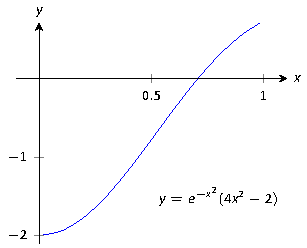
\includegraphics{figures/fignum7a} %Example 138 APEX
\caption{Graphing $f''(x)$ in Example \ref{eg:5.6.4} to help establish error bounds.}
\label{F:5-6-EG4a}
\end{marginfigure}

\begin{marginfigure}[2cm] %MARGIN FIGURE
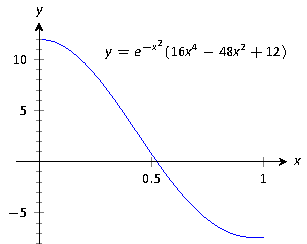
\includegraphics{figures/fignum7b} %Example 136 APEX
\caption{Graphing $f\,^{(4)}(x)$ in Example \ref{eg:5.6.4} to help establish error bounds.}
\label{F:5-6-EG4b}
\end{marginfigure}


\begin{example} \label{eg:5.6.4} % EXAMPLE
Find the error bounds when approximating $\ds \int_0^1 e^{-x^2}\ dx$ using the Trapezoidal Rule and $5$ subintervals, and using Simpson's Rule with $4$ subintervals.

\solution \noindent \textbf{Trapezoidal Rule with $n=5$:}

We start by computing the $2^\text{nd}$ derivative of $f(x) = e^{-x^2}$: $$\fpp(x) = e^{-x^2}(4x^2-2).$$ Figure \ref{F:5-6-EG4a} shows a graph of $\fpp(x)$ on $[0,1]$. It is clear that the largest value of $\fpp$, in absolute value, is $2$. Thus we let $M=2$ and apply the error formula.

$$E_T = \frac{(1-0)^3}{12\cdot 5^2}\cdot 2 = 0.00\overline{6}.$$

Our error estimation formula states that our approximation of $0.7445$ found in Example \ref{eg:5.6.2} is within $0.0067$ of the correct answer, hence we know that
$$0.7445-0.0067 = .7378 \leq \int_0^1e^{-x^2}\ dx \leq 0.7512 = 0.7445 + 0.0067.$$ We had earlier computed the exact answer, correct to $4$ decimal places, to be $0.7468$.\\

\noindent\textbf{Simpson's Rule with $n=4$:}

We start by computing the $4^\text{th}$ derivative of $f(x) = e^{-x^2}$: $$f\,^{(4)}(x) = e^{-x^2}(16x^4-48x^2+12).$$ Figure \ref{F:5-6-EG4b} shows a graph of $f\,^{(4)}(x)$ on $[0,1]$. It is clear that the largest value of $f\,^{(4)}$, in absolute value, is $12$. Thus we let $M=12$ and apply the error formula.

$$E_s = \frac{(1-0)^5}{180\cdot 4^4}\cdot 12 = 0.00026.$$

Our error estimation formula states that our approximation of $0.7468\overline{3}$ found in Example \ref{eg:5.6.3} is within $0.00026$ of the correct answer, hence we know that
$$0.74683-0.00026 = .74657 \leq \int_0^1e^{-x^2}\ dx \leq 0.74709 = 0.74683 + 0.00026.$$ 
\end{example}

 %EXAMPLE
 
%--------------
% SUMMARY
%--------------
\begin{summary}
  \item For a definite integral such as $\int_0^1 e^{-x^2} \, dx$ when we cannot use the First Fundamental Theorem of Calculus because the integrand lacks an elementary algebraic antiderivative, we can estimate the integral's value by using a sequence of Riemann sum approximations.  Typically, we start by computing $L_n$, $R_n$, and $M_n$ for one or more chosen values of $n$.
  \item The Trapezoid Rule, which estimates $\int_a^b f(x) \, dx$ by using trapezoids, rather than rectangles, can also be viewed as the average of Left and Right Riemann sums.  That is, $T_n = \frac{1}{2}(L_n + R_n)$.  
  \item The Midpoint Rule is typically twice as accurate as the Trapezoid Rule, and the signs of the respective errors of these rules are opposites.  Hence, by taking the weighted average $S_n = \frac{2M_n + T_n}{3}$, we can build a much more accurate approximation to $\int_a^b f(x) \, dx$ by using approximations we have already computed.  The rule for $S_n$ is known as Simpson's Rule, which can also be developed by approximating a given continuous function with pieces of quadratic polynomials.
\end{summary}

\clearpage

%--------------
% EXERCISES
%--------------
\begin{adjustwidth*}{}{-2.25in}
\textbf{{\large Exercises}}
\setlength{\columnsep}{25pt}
\begin{multicols*}{2}
\noindent Terms and Concepts \small
\begin{enumerate}[1)]
\item T/F: Simpson's Rule is a method of approximating antiderivatives.
\item What are the two basic situations where approximating the value of a definite integral is necessary?
\item Why are the Left and Right Hand Rules rarely used?
\end{enumerate} 

\noindent {\normalsize Problems} \small

\noindent{\bf In exercises 4--11, a definite integral is given.
\ba
\item Approximate the definite integral with $T_4$.
\item Approximate the definite integral with $S_4$.
\item Compute the exact value of the integral.
\ea}

\begin{enumerate}[1),resume]
\item $\ds \int_{-1}^1 x^2\ dx$
\item $\ds \int_{0}^{10} 5x\ dx$
\item $\ds \int_{0}^{\pi} \sin x\ dx$
\item $\ds \int_{0}^{4} \sqrt x\ dx$
\item $\ds \int_{0}^{3} (x^3+2x^2-5x+7)\ dx$
\item $\ds \int_{0}^{1} x^4\ dx$
\item $\ds \int_{0}^{2\pi} \cos x\ dx$
\item $\ds \int_{-3}^{3} \sqrt{9-x^2} \ dx$
\end{enumerate}

\noindent{\bf In exercises 12--19, approximate the definite integral with $T_6$ and $S_6$.}

\begin{enumerate}[1),resume]
\item $\ds \int_{0}^{1} \cos \big(x^2\big) \ dx$
\item $\ds \int_{-1}^{1} e^{x^2} \ dx$
\item $\ds \int_{0}^{5} \sqrt{x^2+1} \ dx$
\item $\ds \int_{0}^{\pi} x\sin x \ dx$
\item $\ds \int_{0}^{\pi/2} \sqrt{\cos x} \ dx$
\item $\ds \int_{1}^{4} \ln x \ dx$
\item $\ds \int_{-1}^{1} \frac{1}{\sin x+2} \ dx$
\item $\ds \int_{0}^{6} \frac{1}{\sin x+2} \ dx$
\end{enumerate}

\noindent{\bf In exercises 20--23, find $n$ such that the error in approximating the definite integral is less than $0.0001$ using $T_n$ and $S_n$.}

\begin{enumerate}[1),resume]
\item $\ds \int_{0}^{\pi} \sin x \ dx$
\item $\ds \int_{1}^{4} \frac{1}{\sqrt x} \ dx$
\item $\ds \int_{0}^{\pi} \cos \big(x^2\big) \ dx$
\item $\ds \int_{0}^{5} x^4 \ dx$
\end{enumerate}

\noindent{\bf In exercises 24--25, a region is given.  Find the area of the region using Simpson's Rule:
\ba
\item where the measurements are in centimeters, taken in $1$ cm increments, and
\item where the measurements are in hundreds of yards, taken in $100$ yd increments.
\ea}

\begin{enumerate}[1),resume]
\item {\begin{minipage}{\linewidth}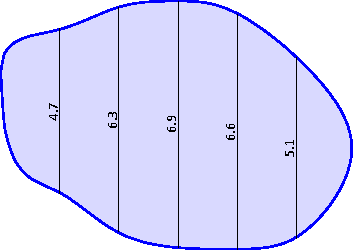
\includegraphics[scale=1]{figures/fig05_05_ex_01}\end{minipage}}

\item {\begin{minipage}{\linewidth}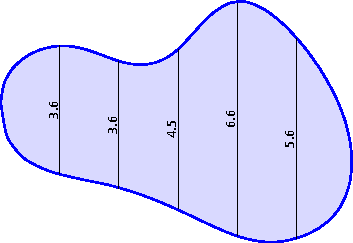
\includegraphics[scale=1]{figures/fig05_05_ex_02}\end{minipage}}

  \item Consider the definite integral $\int_0^1 x \tan(x) \, dx$.
  \ba
  	\item Explain why this integral cannot be evaluated exactly by using either $u$-substitution or by integrating by parts.
	\item Using 4 subintervals, compute $L_4$, $R_4$, $M_4$, $T_4$, and $S_4$.  
	\item Which of the approximations in (b) is an over-estimate to the true value of $\int_0^1 x \tan(x) \, dx$?  Which is an under-estimate?  How do you know?
  \ea
\end{enumerate}

%------------------------------------------
% END OF EXERCISES ON FIRST PAGE
%------------------------------------------
\end{multicols*}
\end{adjustwidth*}

\clearpage

\begin{adjustwidth*}{}{-2.25in}
\setlength{\columnsep}{25pt}
\begin{multicols*}{2}\small

\begin{enumerate}[1),start=27]
  \item For an unknown function $f(x)$, the following information is known.  
  \begin{itemize}
  	\item $f$ is continuous on $[3,6]$;
	\item $f$ is either always increasing or always decreasing on $[3,6]$;
	\item $f$ has the same concavity throughout the interval $[3,6]$;
	\item As approximations to $\int_3^6 f(x) \, dx$, $L_4 = 7.23$, $R_4 = 6.75$, and $M_4 = 7.05$.
  \end{itemize}
  \ba
  	\item Is $f$ increasing or decreasing on $[3,6]$?  What data tells you?
	\item Is $f$ concave up or concave down on $[3,6]$?  Why?
	\item Determine the best possible estimate you can for $\int_3^6 f(x) \, dx$, based on the given information.
  \ea
  
    \item The rate at which water flows through Table Rock Dam on the White River in Branson, MO, is measured in thousands of cubic feet per second (TCFS).  As engineers open the floodgates, flow rates are recorded according to the following chart.
  \begin{center}
\begin{tabular}{|l|c|c|c|c|c|c|c|}
\hline
seconds, $t$ & 0 & 10 & 20 & 30 & 40 & 50 & 60 \\
\hline
flow in TCFS, $r(t)$ & 2000 & 2100 & 2400 & 3000 & 3900 & 5100 & 6500 \\
\hline
\end{tabular}
\end{center}
	\ba
		\item What definite integral measures the total volume of water to flow through the dam in the 60 second time period provided by the table above?
		\item Use the given data to calculate $M_n$ for the largest possible value of $n$ to approximate the integral you stated in (a).  Do you think $M_n$ over- or under-estimates the exact value of the integral?  Why?
		
		\item Approximate the integral stated in (a) by calculating $S_n$ for the largest possible value of $n$, based on the given data.
		
		\item Compute $\frac{1}{60} S_n$ and $\frac{2000+2100+2400+3000+3900+5100+6500}{7}$.  What quantity do both of these values estimate?  Which is a more accurate approximation?
	\ea
\end{enumerate}

%---------------------------------------------
% END OF EXERCISES ON SECOND PAGE
%---------------------------------------------
\end{multicols*}
\end{adjustwidth*}

\afterexercises 

\cleardoublepage